\documentclass{bioinfo}
%\usepackage{amsmath}
%\usepackage{enumerate}
\usepackage{graphicx}
%\author{R.Y.~Neches \& E.G.~Wilbanks} 
%\title{Analyzing ChIP-seq data with Pique}

%\addtolength{\oddsidemargin}{-.875in}
%\addtolength{\evensidemargin}{-.875in}
%\addtolength{\textwidth}{1.75in}
%\addtolength{\topmargin}{-.875in}
%\addtolength{\textheight}{1.75in}

\copyrightyear{2011}
\pubyear{2011}

% This writeup is intended to be submitted to Bioinformatics as an
% Applicaiton Note under either the Gene Expression or Sequence
% Analysis. These are the instructions to authors :
%
% Application Notes (up to 2 pages; this is approx. 1300 words or 1000
% words plus one figure) : Applications Notes are short descriptions
% of novel software or new algorithm implementations, databases and
% network services (web servers, and interfaces). Software or data
% must be freely available to non-commercial users. Availability and
% Implementation must be clearly stated in the article. Authors must
% also ensure that the software is available for a full TWO YEARS
% following publication. Web services must not require mandatory
% registration by the user. Additional Supplementary data can be
% published online-only by the journal. This supplementary material
% should be referred to in the abstract of the Application Note. If
% describing software, the software should run under nearly all
% conditions on a wide range of machines. Web servers should not be
% browser specific. Application Notes must not describe trivial
% utilities, nor involve significant investment of time for the user
% to install.
%
% Software : If the manuscript describes new software tools or the
% implementation of novel algorithms the software must be freely
% available to non-commercial users at the time of submission, and
% appropriate test data should be made available. Availability must be
% clearly stated in the article. Authors must also ensure that the
% software and test data is available for a full TWO YEARS following
% publication. The editors of Bioinformatics encourage authors to make
% their source code available and, if possible, to provide access
% through an open source license (see www.opensource.org for
% examples). Authors should make every effort to use URLs that will
% remain stable. At the minimum, authors must provide one of:
% webserver, source code or binary.
%
% http://www.oxfordjournals.org/our_journals/bioinformatics/

\begin{document}
\firstpage{1}

\title[In a fit of pique]{Analyzing microbial ChIP-Seq data with
  Pique} \author[Neches
\textit{et~al}]{R.Y.~Neches\,$^{1,3}$\footnote{to whom correspondence
    should be addressed}, E.G.~Wilbanks\,$^{1,3}$ and
  M.T.~Facciotti\,$^{2,3}$
  \address{$^{1}$Microbiology Graduate Group, University of California, Davis.\\
    $^{2}$Department of Biomedical Engineering, University of
    California, Davis.\\$^{3}$Genome Center, University of California,
    Davis.}}

\history{Received on XXXXX; revised on XXXXX; accepted on XXXXX}

\editor{Associate Editor: XXXXXXX}

\maketitle

\newcommand{\imsize}{1.0\columnwidth}
%\newcommand{\threeup}{0.26\columnwidth}
%\newcommand{\cotwo}{$\text{CO}_{2}$}
%\newcommand{\htwo}{$\text{H}_2$}
%\newcommand{\otwo}{$\text{O}_2$}
%\newcommand{\water}{$\text{H}_2\text{O}$}
%\newcommand{\htwos}{$\text{H}_2\text{S}$}

\begin{abstract}
\section{Motivation:}

\noindent Most ChIP-Seq peak finders are designed to identify
protein-DNA binding events in eukaryotic datasets. To make
cost-effective use of current sequencing capacity, the peak finders
must be cleverly optimized to work with sparse-coverage data, and must
take into account the effect of chromatin structure on the variation
in background coverage. While numerous effective peak finders have
been developed for eukaryotic systems, the approaches used can be
suprisingly error prone in our hands when run on high-coverage
bacterial and archaeal ChIP-Seq datasets.

% Why not? Examples, evidence, hypothesis. 

\section{Results:}

\noindent Fortunately, many of the statistical challenges for peak
detection inherent in eukaryotic ChIP-seq data are not present in
bacterial and archaeal datasets. This is due in part to higher genome
coverage (typically in inverse proportion to genome size) and in part
to the absence of non-random coverage variation from to highly
structured chromatin.  We have developed Pique, a conceptually simple,
easy to use ChIP-Seq peak finding application for bacterial and
archaeal ChIP-Seq data. The software is cross-platform and Open
Source, and based on Open Source dependencies. Output is provided in
standard GFF files, and easily imported into the Gaggle Genome Browser
for manual curation and data exploration.

\section{Availability:} 

\noindent The software is available under the BSD-3 license at

\href{http://github.com/ryneches/pique}{http://github.com/ryneches/pique}.

\noindent A tutorial and test data are included with the documentation.

\section{Contact:} \href{ryneches@ucdavis.edu}{ryneches@ucdavis.edu}

\end{abstract}

\section{Introduction}

\noindent Next generation sequencing coupled with chromatin
immuno\-pre\-cipi\-tation (ChIP-Seq) is revolutionizing our abilty to
genomically map protein-DNA associations for a wide variety of
proteins.  The growing popularity of ChIP-Seq has spurred the
development of over thirty peak picking algorithms (for a nearly
completely list see \cite{wilbanks}). The relative performance of
represetative peak detection algorithms on eukatyoric data and methods
to assess performance have been recently reviewed by several authors
\cite{Pepke, Laajala_review, too_many_peak_callers, peakranger,
  peak_benchmark}.  Many of these peak picking methods have employed a
number of sophisticated strategies to detect peaks in the typically
sparsely covered eukaryotic datasets for which they are designed.

While ChIP-Seq has been predominantly used to interrogate protein-DNA
interactions in eukaryotic systems, there are clear advantages to
adopting this technology for studying microbial systems. Microbial
genomes typically are much smaller than eukaryotic genomes (the genome
of {\em E. coli} is $\approx$2000 times smaller than the human
genome), and have simpler replicon and chromatin structure.  We were
surprised to find that software that works well in eukaryotic systems
tends to fail when presented with an presumably lesser challenge.

To our knowledge, only one other peak finding package, CSDeconv
\cite{CSDeconv}, has been explicitly developed for finding peaks in
microbial ChIP-Seq data. This MATLAB package successfully finds peaks
in microbial ChIP-Seq data, but its application is limited by its
dependency on costly proprietary software, slow performance, lack of
support for manual curation, and high false negative rate. Herein we
describe Pique, a conceptually simple, Python-based peak finding
package that enables easy and rapid peak finding in bacterial and
archaeal ChIP-Seq datasets.

\section{Approach}

\noindent ChIP-Seq in bacteria and archaea yields coverage several
orders of magnitude larger than in eukaryotic systems.  This generates
data with continuous signal across the microbial chromosome rather
than the sparse coverage typically present in eukaryotic ChIP-Seq
data.  This feature of microbial ChIP-Seq data permits simpler, faster
algorithms to be used. We have based our algorithm on classic noise
reduction techniques from signal processing.

Pique is designed for use in systems that have genomic complexities
such as IS elements, gene dosage polymorphisms and accessory genomes
that cause variations in sequence coverage unrelated to ChIP, or in
cases where the organism under study is not identical to the reference
genome. The resulting enrichment ``pedestals'' and ``holes'' can be
very problematic for detecting peaks and calculating enrichment
levels. Pique allows the user to optionally supply a map of these
features as a GFF file, and the software will automatically perform a
segmented analysis.

Pique has integrated curation support through the Gaggle Genome
Browser. This permits interactive curation of the peak list and
analysis of the ChIP-Seq data in the context of other Gaggle-enabled
resources. Interactive curation of a microbial ChIP-Seq data set can
typically be completed in a few minutes.

\begin{methods}
\section{Methods}

\noindent Prior to running Pique, Illumina (Solexa) reads should be
quality filtered, quality trimmed, and aligned to a reference genome
using the user's preferred short-read sequence aligner. Pique requires
a BAM file as input \cite{sam_format}. We suggest using all contigs of
the reference genome as the mapping target, but the user may prefer to
proceed with one contig at a time if desired.

The user may optionally supply a map of coverage features. Pique
supports three features; analysis regions, exclusion regions, and
normalization regions. By default, Pique treats each contig as a
single analysis regions, but the user may designate regions within a
contig for separate analysis. This is useful where a gene dosage
polymorphism has systematically altered the coverage level in a large
region. Exclusion regions are simply masked out of their respective
analysis regions, and are useful for removing coverage variation due
to repetitive DNA. If the user designates normalization regions within
an analysis region, Pique will use them to compensate for total coverage
discrepancies between the background and ChIP alignments.

The user launches the primary analysis stage by providing alignment an
file for the ChIP data, an alignment file for the control data, and
optional an coverage feature map. The primary analysis proceeds thusly
:

\begin{itemize}

\item The alignment files are digested, and the analysis regions are
  initialized. If a coverage feature map provided, the analysis
  regions are separated and the exclusion regions applied.

\item The coverage noise threshold is measured by comparing the
  relative total coverage within the normalization regions. (The user
  should choose normalization regions that contain neither peaks nor
  coverage level aberrations.)

% This no longer happens in the current version, as of August 18, 2011
%
%\item In each analysis region, the ``DC'' component is removed using
%  linear detrending. This removes effects due to coverage variation
%  features larger than about 100Kb.

\item High-$k$ noise in coverage is removed using a Wiener-Kolmogorov
  filter. The filter delay $\alpha$ is chosen to approximate to the
  expected footprint size of the targeted protein. The choice of
  filter implies the existence of two inputs; a ``true'' signal, and a
  noise source. Both are assumed to be stationary stochastic processes
  combined additively.

  % The Wiener-Kolmogorov filter was the first and simplest
  % statistical signal filter, first published by Norbert Wiener in
  % 1949, and independently derived in discrete-time form by Andrey
  % Kolmogorov in 1941.

\item A Blackman window of a diameter equal to the read length is
  convolved with the filtered coverage track to remove features
  smaller than one read. 

\item The noise threshold in the ChIP coverage track is measured by
  comparing the coverage distribution in the ChIP track to the control
  track within user-annotated non-peak regions. Features that exceed
  the noise threshold are identified.

\item To determine if a feature corresponds to a binding event, we
  require that the stop coordinate of the forward strand enrichment
  envelope must fall between the coordinates of the reverse strand
  enrichment envelope, and that the start coordinate of the reverse
  strand enrichment envelope fall between the coordinates of the
  forward strand enrichment envelope. (We call this the overlap
  criterion.)

\end{itemize}

% FIXME : The overlap criterion is a very crude version of the
% heuristic models other peak callers user. We should say something
% here about these models, and why decided not to use them.

\noindent For each putative peak, the enrichment ratio of the ChIP
alignment to the the control alignment, estimates the binding
coordinate, and reports to the user, as well as the enrichment
normalization factor for that analysis region are calculated and
compiled into user output.  Determination of the statistical
significance of a peak is highly specific to the experiment, and so
Pique does not undertake this calculation.

\end{methods}

\begin{figure}[!tfbd peak - a nice one]%figure1
  % \centerline{\includegraphics{example_data.png}
  \begin{center}
    {\resizebox{\imsize}{!}{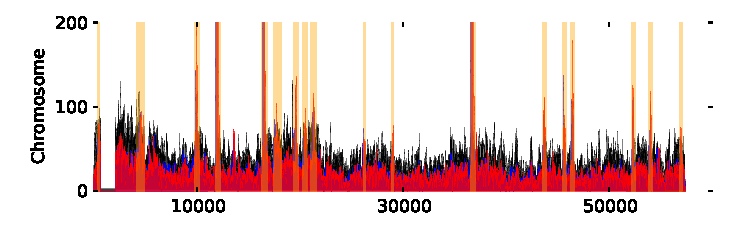
\includegraphics{chr_example.pdf}}}
    %{\resizebox{\imsize}{!}{\includegraphics{../PNRC200_0:21851.pdf}}}
    %{\resizebox{\imsize}{!}{\includegraphics{../PNRC200_47121:88549.pdf}}}
  \end{center}
  \caption{Peaks found in the chromosome of the included sample
    dataset, derived from ChIP-seq of tfbD in {\em Halobacterium
      salinarum} sp. NRC1. Blue and red indicate coverage of reads
    aligned from the ChIP-derived data to the forward and reverse
    strands of the genome, respectively. Black indicates coverage
    aligned from the whole cell extract data. Orange indicates a
    detected peak. The maximum coverage in this data is 3204, but is
    shown here truncated at 200.}\label{fig:01}
\end{figure}

\begin{figure}[!tfbd data - reasonable spot showing curation]%figure2
  \begin{center}
    {\resizebox{\imsize}{!}{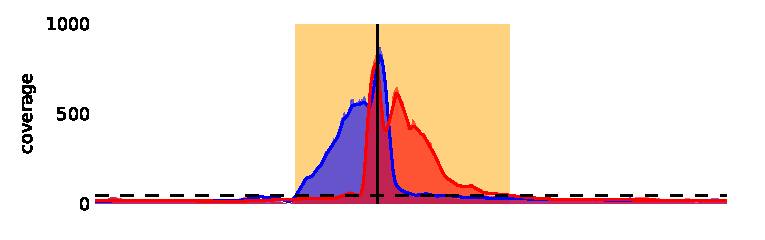
\includegraphics{peak_example.pdf}}}
    {\resizebox{\imsize}{!}{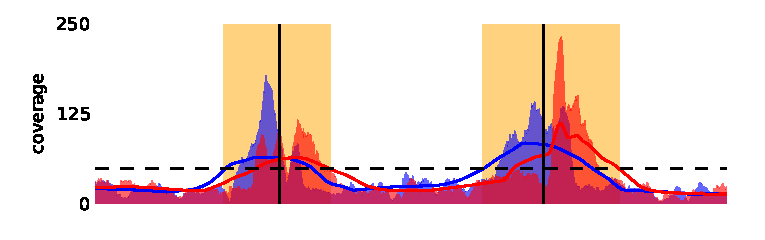
\includegraphics{peak_example_2.pdf}}}
  \end{center}
  \caption{Examples of large and medium-size peaks.}\label{fig:02}
\end{figure}

\section{Discussion}

The coverage enrichment is distributed differently between the forward
and reverse strands due to the constrained read orientation imposed by
the fragment size.

Pique does not attempt to filter peaks that are statistically
insignificant. We have found that this part of the analysis is rather
specific to the data and to the experiment. Pique is designed to
achieve a low false-negative rate, which comes at the cost of a
relatively high false-positive rate. Thus, some kind of post-filtering
is necessary. Pique provides the user with output that can be used to
support a variety of such statistical tests.

Some recommended filtering might include :

\begin{itemize}
\item Eliminate peaks that are significantly narrower than the size
  range of the sequencing library.
\item Eliminate peaks with a normalized enrichment ratio below unity.
\item Eliminate peaks that have predicted binding sites that are very
  skewed from the center of the enriched region.
\end{itemize}

Depending on how many peaks are recovered, the user may wish to try
one or all of these, perhaps with clustering. However, if a
``perfect'' peak list is required, we do not recommend relying on
statiastical refinements alone. To facilitate manual curation, Pique
outputs a track file of the coverage, a quantitative positional data
of the estimated binding sites, and a bookmark file annotating the
peaks. These files are simple to process by a variety of tools, and
can be loaded directly into the Gaggle Genome Browser.\footnote{See
  supplementary figure.}

\section{Conclusion}

We note that Pique should also work well with eukaryotic datasets
provided they are gathered with greater coverage than has been
previously reported.

\section*{Acknowledgement}
\paragraph{Funding\textcolon} 

This project was funded by UC Davis startup funds to MTF, NSF graduate
fellowship AWARD NUMBER to EGW and DARPA AWARD NUMBER TO RN.

%\bibliographystyle{natbib}
%\bibliographystyle{achemnat}
%\bibliographystyle{plainnat}
%\bibliographystyle{abbrv}
%\bibliographystyle{bioinformatics}

\bibliographystyle{plain}

\bibliography{writeup}

\end{document}